% LaTeX file
\documentclass[11pt]{article}
\usepackage{amsmath}
\usepackage{amssymb}
\usepackage{amsthm}
\usepackage{graphicx}
\usepackage{natbib}
\usepackage{tikz}
\usetikzlibrary{calc,patterns,decorations.pathmorphing,decorations.markings}

\title{Physics Behind the Simulation: A CS296 Report by Group 19}
\author{Abhinav Gupta (120050029) \\ abhinav@cse.iitb.ac.in \\ Anant Gupta (120050086) \\anant@cse.iitb.ac.in\\ Stephan Biastoch (13V051004)\\sbiastoch@cse.iitb.ac.in}
\date{January 25, 2014}

\begin{document}
\maketitle

\section{Introduction}
This report explains the modification of the Box2D base code provided for the Software Systems lab. Box2D is a 2 dimensional Physics Simulation Engine where a variety of objects and situations can be created. Three new objects have been added to the base code and are described in the following report.
\pagebreak

\section{Physics behind the simulation}

Following are the new additions in the original setup:
\begin{itemize}
\item[1] Projectile Hitting the Pendulum
\item[2] A Long Light Block
\item[3] A ball hitting the light block and the open box
\end{itemize}

They have been described in the following subsections.

\pagebreak

\subsection{Projectile Hitting the Pendulum}


The Pendulum has been modified to start from the mean position. So, to start the domino effect a projectile strikes the pendulum setting it into motion.\\

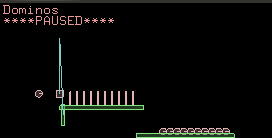
\includegraphics[scale=0.7,natwidth=272,natheight=138]{11.png}

\begin{align}
m_1u_1 = m_1v_1 + m_2v_2
\end{align}
\begin{align}
eu_1 = v_2 - v_1
\end{align}
where,\\
$m_1$ is the mass of projectile,\\
$m_2$ is the mass of pendulum,\\
$u_1$ is the initial velocity of projectile,\\
$v_1$ is the velocity of projectile after collision,\\
$v_2$ is the velocity of pendulum after collision and\\
$e$ is the coefficient of restitution.\\

After the collision: \\

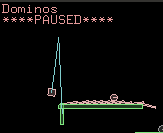
\includegraphics[scale=0.7,natwidth=163,natheight=133]{./12.png}

\pagebreak

\subsection{A Long Light Block}
A long light block has been introduced to strike the above mentioned projectile so that it moves out of the way of the pendulum.\\

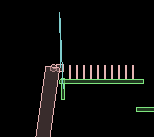
\includegraphics[scale=0.7,natwidth=154,natheight=137]{./21.png}

The block has some initial vertical velocity and a small angular velocity. 

The block is also hit by a ball and after some rather hilarious collisions moves out of the pictures.\\

\begin{align}
I\omega_1 + mv_1r = I\omega_2 + mv_2r 
\end{align}

\begin{align}
MV_1 + mv_1 = MV_2 + mv_2
\end{align}
where,\\
$I$ is the moment of inertia of block,\\
$\omega_1$ is the initial angular velocity of the block,\\
$\omega_2$ is the angular velocity of the block after collision,\\
$V_1$ is the initial velocity of center of mass of block,\\
$V_2$ is the velocity of center of mass of block after collision,\\
$v_1$ is the initial velocity of ball,\\
$v_2$ is the velocity of ball after collision,\\
$M$ is the mass of the block, and\\
$m$ is the mass of the ball.\\
\cite{hcv}\\

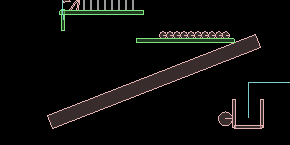
\includegraphics[scale=0.7,natwidth=290,natheight=145]{./22.png}

\pagebreak

\subsection{A ball hitting the light block and the open box}

This ball serves a multifold purpose. 

First, the ball hits the light box and the box moves out of the picture.\\

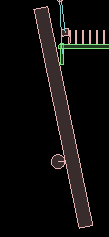
\includegraphics[scale=0.7,natwidth=109,natheight=237]{./31.png}

Second, the ball hits the open box and puts it in to an oscillatory motion so that the falling of the small spheres into the box becomes unpredictable (and interesting to watch).\\

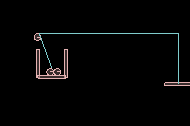
\includegraphics[scale=0.7,natwidth=190,natheight=126]{./32.png}

Third, the ball after creating the aforementioned nuisance settles under the inclined plank.
On impact from the heavy sphere the light box on the plank jumps up and this ball flies away through the gap.\\

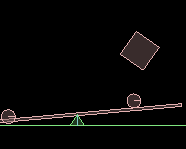
\includegraphics[scale=0.7,natwidth=186,natheight=149]{./33.png}

\pagebreak

\section{Conclusion}

All in all, the introduction of the three new elements creates variety which threatens to hamper the normal domino movement but fortunately (or mathematically?) it is unaffected.

\bibliographystyle{te}
\bibliography{references}

\end{document}
